%!TEX root = thesis.tex

%:-------------------------- Preamble -----------------------

% Three languages are supported, which will be reflected in the logo on the front page. Pass the appropriate language
% specified as a class option to uit-thesis. Passing any other languages supported by babel will result in the default
% language on the frontpage. If no language is passed, the default is selected.
%  - USenglish (default)
%  - norsk
%  - samin
% The frontpage comes in two variants, Master's thesis and PhD. Master is default, use classoption 'phd' for the PhD version.
\documentclass[USenglish]{uit-thesis}


% Lorem ipsum
%\usepackage{lipsum}

\makeglossaries

% Add external glossaryentries
\loadglsentries{acronyms}
\newacronym{api}{API}{application programming interface}\glsunset{api}
\newacronym{2api}{2API}{application programming interface}
\newacronym{d3}{D3}{Data-Driven Documents}
\newacronym{html5}{HTML5}{version 5 of the HyperText Markup Language standard}
\newacronym{wsn}{WSN}{Wireless Sensor Network}
\newacronym{bs}{BS}{Base Station}
\newacronym{ch}{CH}{Cluster Head}
\newacronym{coat}{COAT}{Climate-ecological Observatory for Arctic Tundra}
\newacronym{ou}{OU}{Observation Unit}
\newacronym{leach}{LEACH}{Low-Energy Adaptive Clustering Hierarchy}
\newacronym{fleach}{F-LEACH}{Fuzzy-LEACH}
\newacronym{gbcp}{GBCP}{Gossip-based communication protocol}
\newacronym{pegasis}{PEGASIS}{Power-efficient gathering in sensor information systems}


\newglossaryentry{thesis}
{
  name=thesis,
  description={is a document submitted in support of candidature for an
    academic degree or professional qualification presenting the author's research and findings},
}
\newglossaryentry{lage}
{
  name={long ass glossary entry},
  description={is a long ass entry with a lot of text describing the properties of the glossary entry. Hopefully this spans some lines now.},
}


\newcommand{\listdefinitionname}{My list of definitions}
\newlistof{definition}{def}{\listdefinitionname}
\newcommand{\definition}[1]{%
  \refstepcounter{definition}%
  \par\noindent\textbf{The Definition~\thedefinition. #1}%
  \addcontentsline{def}{definition}
    {\protect\numberline{\thechapter.\thedefinition}#1}\par%
}

\begin{document}

%:-------------------------- Frontpage ------------------------

\title{Peer Observations of Observation Units}
%\subtitle{Subtitle}			% Optional
\author{Camilla Stormoen}
\thesisfaculty{Faculty of Science and Technology \\ Department of Computer Science}
\thesisprogramme{INF-3981 Master's Thesis in Computer Science ... May 2018}
%\ThesisFrontpageImage{example_image.jpg}	% Optional

\maketitle

%:-------------------------- Frontmatter -----------------------
\frontmatter

%\begin{dedication}
%To Leslie.
%Fuck you very much.
%\end{dedication}


%\begin{epigraph}
%\epigraphitem{Simplicity is prerequisite for reliability.}{Edsger Dijkstra}
%\epigraphitem{Beware of bugs in the above code;\\I have only proved it correct, not tried it.}{Donald Knuth}
%\end{epigraph}


\begin{abstract}
What is wrong with the world? Motivation 1-3 sentences, Arch, Des, Imp, Exp 1,2-3 sentences, results and main conclusion.
\end{abstract}

\begin{acknowledgement}
%First I would like to thank my main advisor Professor Otto Anshus and co-advisor Associate Professor John Markus Bjørndalen for providing guidance, support, ideas and feedback whenever I needed it through this thesis.

%I want to express my sincerest gratitude to the \textit{Masterinos}. I would not have made it without you guys. 

%I would also like to thanks my parents for encouraging me to take a higher education and supporting me through every decision. A great thanks to my boyfriend
\end{acknowledgement}

\tableofcontents

%\listofdefinition

%\listoflistings

\printglossary
%\printglossary[type=\acronymtype]
%\printglossaries


%:-------------------------- Mainmatter -----------------------
\mainmatter

\chapter{Introduction}
\textbf{FRA CAPSTONE:}
\textit{The Arctic tundra in the far northern hemisphere is challenged by climate changes in the world today and is one of the ecosystems that are most affected by these changes[10]. The \gls{coat} is a long-term research project developed by five Fram Center\footnote{\url{http://www.framsenteret.no/english}} institutions. Their goal is to create robust observation systems which enable documentation and understanding of climate change impacts on the Arctic tundra ecosystems. COAT was in autumn 2015 granted substantial funding to establish research infrastructure which allowed them to start up a research infrastructure during 2016-2020[10].}


\Gls{wsn} is a system that consists of hundreds or thousands of low-cost micro-sensor nodes. These nodes monitor and collect physical and environmental conditions. The various activities  in the sensor nodes consume lots of energy and the battery of the sensor node is difficult to recharge in wireless scenarios and also because the sensor nodes are located at remote areas in the Arctic tundra.

%\Gls{wsn}s main task is to periodically collect information of the interested area and broadcast the information to a \gls{bs}. An easy approach to achieve this task is to make each sensor node transmit their data directly to the BS. But the problem  is that the BS can be far away from the sensor node and the sensor node will die due to energy consumption.

%It is beneficial to make these sensors as cheap and energy-efficient as possible.

\textit{This thesis presents the architecture, design and implementation of a peer observation that can observe and accumulate data from in-situ observation units.}

\section{Motivation}
The motivation behind this project is...


%This project will develop an approach to 
%\begin{itemize}
%\item Let observation units observe data observed by observation units. 
%\item To gradually accumulate the data to observation units being a DAO Store (there can be multiple DAO Stores depending on user needs).
%\item Do a prototype of such a system focused on three levels of observation units: (i) In-situ observation units being (ii) observed by back-end observation units, being (iii) observed by a DAO Store observation unit.
%\end{itemize}


The purpose is to fetch and accumulate data observed by observation units for further use.

The observation units to be used for the prototype comprises
Observation Unit Processes executing on PCs and/or Raspberry Pi.


\section{Contributions}
The dissertation makes the following contributions:
\begin{itemize}
\item A
\item B
\end{itemize}

\section{Assumptions}
Avgrense viktig!

\section{Limitations}
Avgrense viktig!
%Fokus på cluster som tar hensyn til batteri mtp at nodene er ute i tundraen og ikke har mye tilgang til strøm.. redundancy, reliability, scalability?? 
%\paragraph{A paragraph}

\section{Outline}
This thesis is structured into X chapters including the introduction.

\begin{description}
\item[Chapter 2] describes ..
\item[Chapter 3]
\item[Chapter 4]
\item[Chapter 5]
\item[Chapter 6]
\item[Chapter X]
\end{description}


%\subsection{A subsection}
%We can use the \ac{api} to \ac{2api} do stuff, and write about what we did in a \gls{thesis}!

%This is some stuff, {\sc smallcaps {\em smallcapsemphasized}} {\em regularemphasized}

%\Gls{lage}: a test glossary entry.

%If the acronym \ac{uit} is displayed, then loadglsentries works.

%It is fun to use modern \upsc{OpenMP} technology!\footnote{This is a snarky footnote. Words and etc. Semantic web technologies are technologies that enable semantification of the Web as we know it today. Hopefully this spans some lines now.}

%It is fun to use \emph{modern \upsc{OpenMP}} technology! And it is fun to use \ac{d3} and \ac{html5}.

%\definition{Some other definition}




\chapter{Routing Techniques in WSNs?}
Som eget kapittel eller ha det under Related Work? Si noe om routing protocols som hierarchical (evt flat-based og location-based) og si noe om routing protocol operations som multipath (evt. query-based, QoS-based, coherent-based etc..)?

Har også fra WSN-bok ("Protocols and Architectures for Wireless Sensor Networks, Holger Karl, Andreas Willig) kap. 11 som heter "Routing Protocols" som sier noe om gossiping, energ-efficient unicast, broadcast/multicast, geographic routing og mobile nodes..


%\cite{rout_prot_survey}

%\begin{figure}
%\centering
%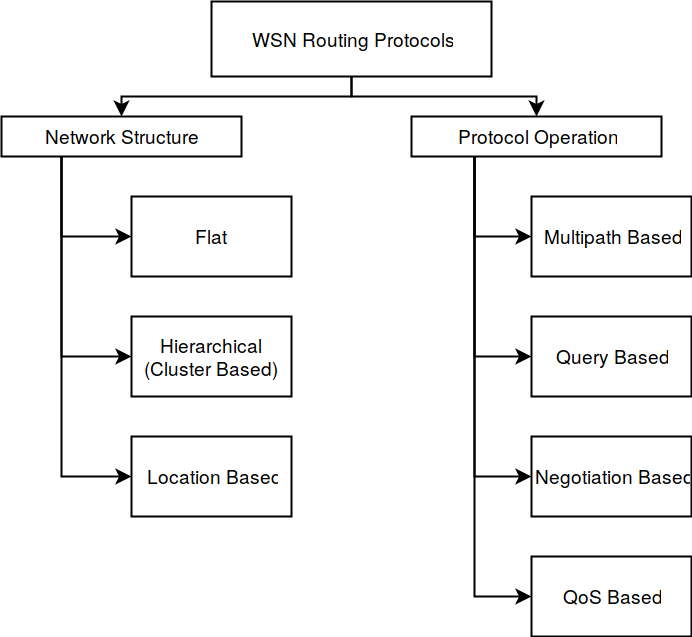
\includegraphics[width=\textwidth]{taxonomy.png}
%\caption{Figure showing taxonomy of routing protocols in WSNs.}
%\label{fig:taxonomy}
%\end{figure}

%\section{Routing Protocols in WSNs}
%\subsection{Flat-based Routing}
%In flat-based routing...

%\begin{itemize}
%\item SPIN
%\item Direct diffusion
%\item Rumor routing
%\item MCFA 
%\item COUGAR
%\item ACQUIRE
%\item Energy-Aware routing
%\end{itemize}


%\subsection{Hierarchical Routing}
%Hierarchical routing is a well know technique for network routing with special advantages related to scalability, efficient communication and energy-efficient routing in WSNs \cite{leach}\cite{leach_perf}.

%\textit{Hierarchical routing is an efficient way to lower energy consumption within a cluster, performing data aggregation and fusion in order to decrease the number of transmitted messages to the \gls{bs}.}

%\begin{itemize}
%\item LEACH
%\item HEED
%\item PEGASIS
%\item TEEN/APTEEN
%\end{itemize}

%\subsection{Location-based Routing}
%In location-based routing are the nodes addressed by means of their locations. The distance between neighboring nodes can for example be estimated on the basis of incoming signal strengths or the location of the nodes can be available by using \cite{routing_survey}. 

%\begin{itemize}
%\item GAF
%\item GEAR
%\item MFR, DIR, GEDIR
%\item SPAN
%\end{itemize}

%\section{Routing Protocol Operations}
%\subsection{Multipath Routing Protocol}
%\subsection{Query-based Protocol Operation}
%\subsection{Negotiation-based Protocol Operation}
%\subsection{QoS-based Protocol Operation}
%\subsection{Coherent-based Protocol Operation}


\chapter{Related Work}
%\section{Routing Protocols in WSNs}
\Gls{wsn}s  main task is to periodically collect information of the interested area and broadcast the information to a \gls{bs}. An easy approach to achieve this task is to make each sensor node transmit their data directly to the BS. But the problem is that the \gls{bs} can be far away from the sensor node so a direct data transmission would not be possible, or if the routing path from the sensor node to the \gls{bs} is long, the sensor node may/will die due to energy consumption. There are multiple hierarchical protocols that has been proposed as a solution to this problem.

To improve the overall energy dissipaton of \gls{wsn}s, \gls{leach} \cite{leach} introduce a hierarchical clustering algorithm for sensor networks. It is self-organized and use randomization to distribute the energy load evenly among the sensors in the network. The sensor nodes organize themselves into local clusters where one node is the local \gls{bs} or \gls{ch}. The \gls{ch} are not fixed to avoid nodes to drain their battery and to spread the energy usage over multiple nodes. The nodes self-elect a new \gls{ch} depending on the amount of energy left at the nodes at different time-intervals. \gls{leach} is divided into different rounds where each round include a setup phase and a steady-state phase \cite{tree_based}. In the setup phase will each node decide whether to become a \gls{ch} or not. When a \gls{ch} is chosen, each node will select its own \gls{ch} based on the distance between the node and the \gls{ch} and join the cluster. In the steady-state phase will the \gls{ch} fuse the received data from the node members in the cluster and send it to \gls{bs}.

In diversity, will nodes in our approach first connect to a cluster and then start a \gls{ch} election rather than elect a \gls{ch} first and then nodes joining the cluster. %This is described further in Section/Chapter \ref{xx}.
A resemblance between the two approaches is that neither of them consider a nodes energy level when calculating the \gls{ch}.
%\begin{equation}
%T(n) = \frac{P}{1-P\times(r \bmod \frac{1}{P})}
%\end{equation}

%\begin{equation} \label{eq:leach}
%T(n) = \begin{cases}\frac{P}{1-P\times(r \bmod \frac{1}{P})} & if n \in G
%\\0 & otherwise\end{cases}
%\end{equation}


\gls{leach} do not consider a nodes energy level when calculating the \gls{ch} and has been a benchmark for improving algorithms such as the centralized clustering algorithm LEACH-C \cite {leach_c} and distributed clustering algorithm such as LEACH-E \cite{leach_e} and LEACH-B \cite{leach_b}. They concentrate on energy consumption reducing a nodes residual energy and more relevant criterions \cite{dec_cb_alg}.


%\begin{equation} \label{leach_c}
%P_{i}(t)=\min\left\{\frac{E_{i}(t)}{E_{total}(t)}k, 1\right\}
%\end{equation}

\Gls{fleach} \cite{fuzzy_logic} \cite{ch_fuzzy} have three different fuzzy descriptors such as energy, concentration and centrality used to complement the cluster head selection process. The \gls{bs} performs the \gls{ch} election in each round by computing the chances of a node becoming a \gls{ch} by calculating the three fuzzy descriptors. \Gls{fleach} also assumes that the \gls{bs} elects the appropriate \gls{ch} because it has a complete information about the whole network.

In contrast to \gls{fleach} will our approach elect a \gls{ch} by the nodes in the cluster and not in a \gls{bs}. The \gls{ch} election will not consider "variables" such as battery level or number of nodes in the cluster.


\Gls{pegasis} is a chain-based protocol with the idea to form a chain among the sensor nodes so each node will receive and transmit data to a close neighbor. The sensor nodes will also take turns on being the leader for transmitting data to the \gls{bs} and therefor distribute the energy load evenly among the sensor nodes. The chain can be organized by the nodes themselves using a greedy algorithm starting from some node or the \gls{bs} can compute the chain and broadcast it to all the nodes in the network \cite{pegasis}.

To increase the robustness of devices and lower power consumptions, ZebraNet \cite{zebranet} provides a low-power wireless system for position tracking of wildlife by using peer-to-peer network techniques. This reduces the researchers effort to manage the sensors and collecting logged data for their research. The radios on their devices also operates on different frequencies and have different bandwidth, range and other characteristics.

A diversity to our approach is that ZebraNet stores multiple copies of the same data across multiple nodes while our approach forwards the data to a node

%Compared to our approach, 
%ZebraNet stores multiple copies of the same data across multiple nodes whilist our apporach forward the data to a node which is believed to have the best chance to access a base station..


%"When network nodes have multiple radios, the shortest path algorithm does not perform well". p.1 in paper


%\section{Data Collection/Aggregation in WSNs}
%Di Franscesco et. al. \cite{dataColl}


%\section{Gossip-based Protocols}
Gossip-based protocols, or epidemic protocols, are popular protocols due to their ability to reliably pass information among a large set on interconnected nodes. Jelasity et al. \cite{gbsampling} provide a \gls{gbcp} where each node have peers to gossip with in a large-scale distributed system \cite{demers}. These nodes can quickly join and leave the network at any given point of time. The general principle of their framework is that every node (1) maintains a relatively small local membership table that provides a partial view of all nodes and (2) periodically refreshes the table using a gossiping procedure.

The difference between \gls{gbcp} and our approach is that our approach does not use a gossip protocol to update its table of nodes, but instead relies on the communication with other nodes to know about the election of a new \gls{ch}, which of the node is the \gls{ch} and when a node should accumulate data and send it to the \gls{ch}.


\chapter{Architecture}
%Tell it clean/neat. Abstractions, functionalities

This chapter describes the architecture of the system. The main functionality can be divided into 3 sub-sections: a nodes lookup service, discovery of other nodes and incoming network requests. The architecture of the system is presented in \ref{fig:architecture} (or \ref{fig:architecture3}?).

\begin{figure}
\centering
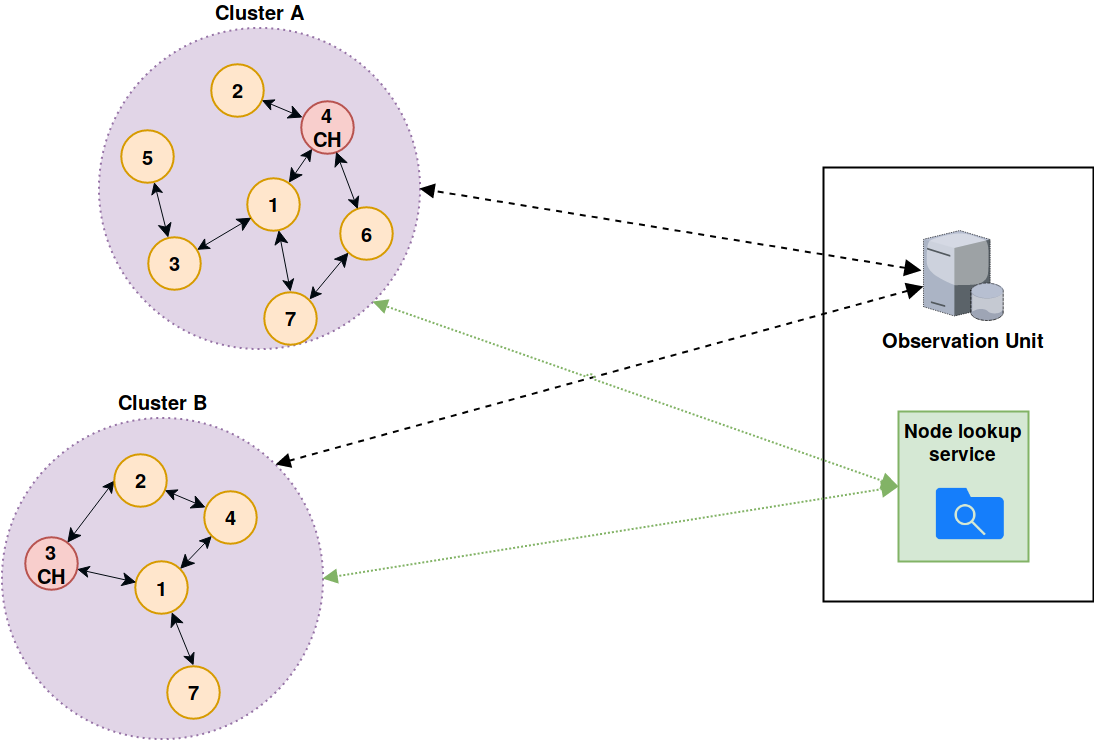
\includegraphics[width=\textwidth]{architecture.png}
\caption{Figure shows the architecture of the system.}
\label{fig:architecture}
\end{figure}


\begin{figure}
\centering
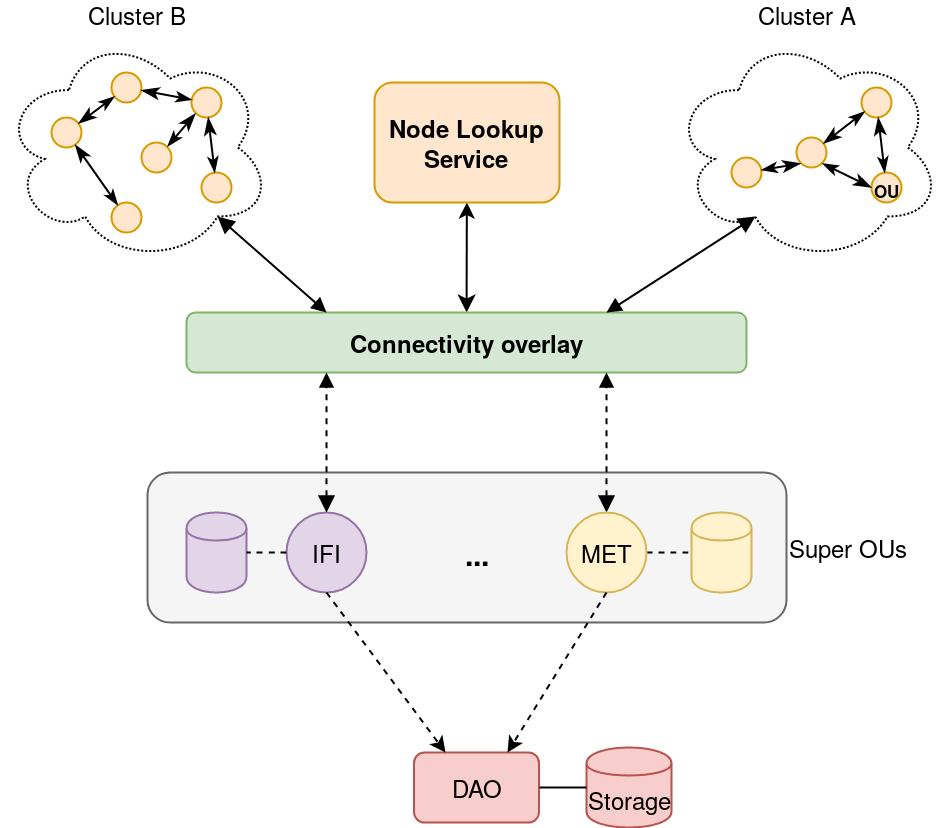
\includegraphics[width=\textwidth]{arch3.png}
\caption{Figure shows the architecture of the system.}
\label{fig:architecture3}
\end{figure}

\section{Node Lookup Service} \label{sec:nodeLS}
The lookup service is responsible for storing a list of all previous discovered nodes and their address.

\section{Discovery Of Other Nodes} \label{sec:discON}
Each node can only discover nodes withing a possible range. Figure \ref{fig:broadcast_range} shows how a possible range of a node may be discovered. When a new node in the network has been discovered will meta-data about the node such as address be stored on locally on the device in the cluster.

\section{Incoming Network Requests}
A node may receive incoming requests from other nodes in the network. The request handler will handle the request based on the type of request. The types of requests a node may receive are listed below.

\subsection{Connect To Neighbours}
When a node receive a list of neighbours in range, it will try to connect to the neighbours that are within the nodes range. It will only connect to the neighbour node if it receives a OK-message.

\subsubsection{Receive OK From Neighbours}
When a node receives a OK-message it will connect itself to the neighbour. The neighbour will also then have connected to the new node.

\subsection{Cluster Head Election Request}
A node may receive a \gls{ch} election request when a node has joined the cluster.

\subsubsection{Cluster Head Election Request}
When a node receives a \gls{ch} election request it will perform a leader election and forward the result to it's neigbours which will do a leader election as well.

\subsubsection{Cluster Head Election Calculation Request}
If there is a leader in the cluster already and a new election should be proposed, a \gls{ch} election calculation request is sent from the leader. Nodes receiving this request will calculate their \gls{ch} election number. This is explained further in Section xx.

\subsection{Data Transmission}
\subsubsection{Notify Neighbours About Sending Data To Leader}
A node may receive a request that it should send its data to the leader. This request is forwarded to the nodes neighbour and so on.

\subsubsection{Send Data To Leader}
This request forwards a nodes data to the next node in the path to the leader. If the nodes data receiving this requests isn't sent to the leader of the cluster, will the data be accumulated with the received data and then forwarded to the next node.

%\section{Base Station Access}
%CH should access BS..?


\chapter{Design}
%Server, p2p, protocols..
In this chapter we will look at the design of the system and present the design of each component of the architecture. Figure \ref{fig:design} shows how the cluster network may appear (in the system). Nodes are connected to other nearby nodes represented by arrows and together they form a cluster network.

\begin{figure}
\centering
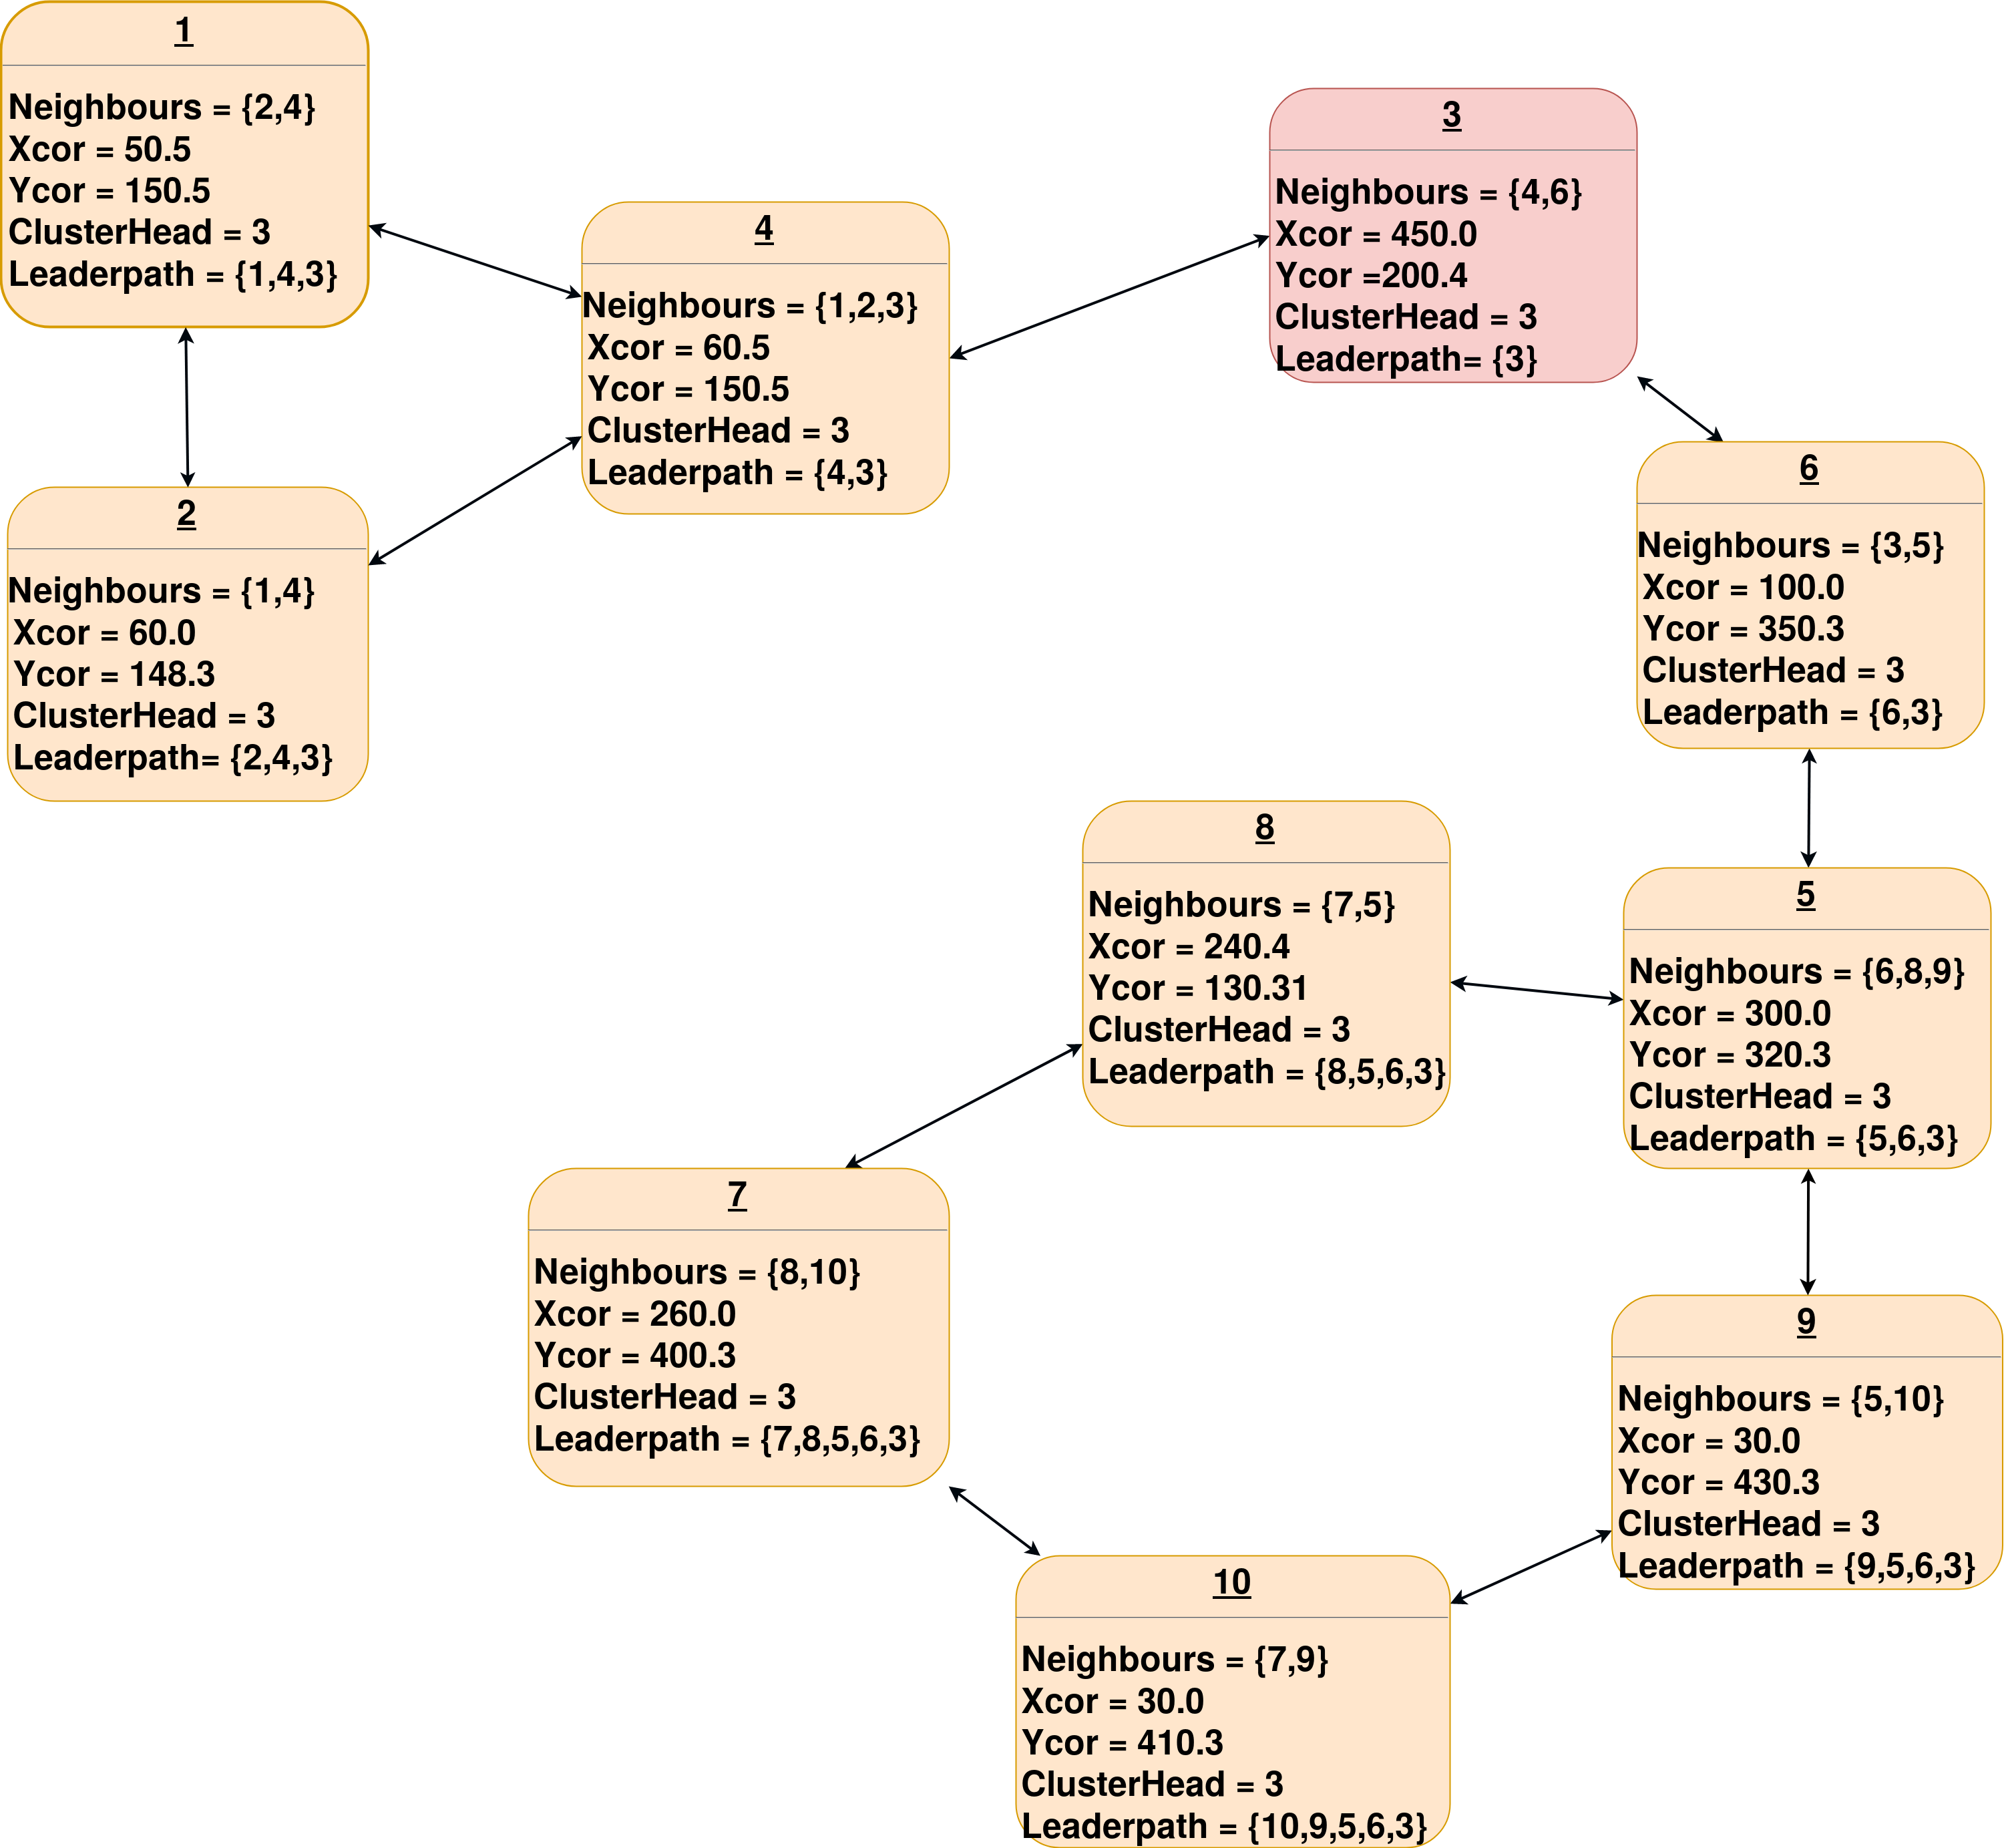
\includegraphics[width=\textwidth]{design.png}
\caption{Figure show design of the system.}
\label{fig:design}
\end{figure}

\section{Discovery Of Other Nodes}
\subsection{Broadcasting}
When a new node start it will contact the node lookup service to discover other nodes in the network. The node will then initiate a broadcast.
Broadcast is limited due to a radio range limitations where only nodes that are within this range will receive the broadcast, shown in Figure \ref{fig:broadcast_range}. \textit{Node 1} will only reach \textit{node 5} and \textit{node 7}.


\begin{figure}
\centering
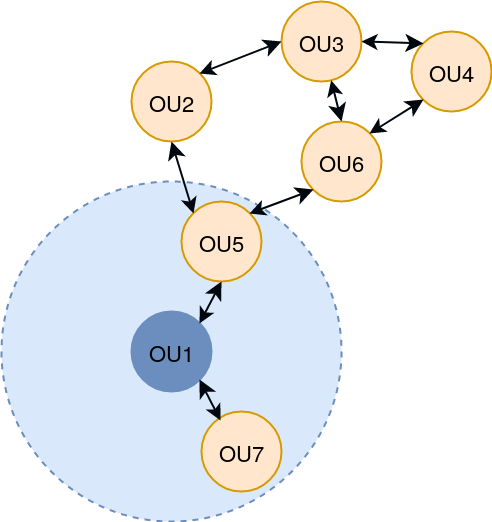
\includegraphics[scale=0.4]{broadcast_range.png}
\caption{Figure show broadcast range of a \gls{ou}.}
\label{fig:broadcast_range}
\end{figure}


%\begin{figure}
%\centering
%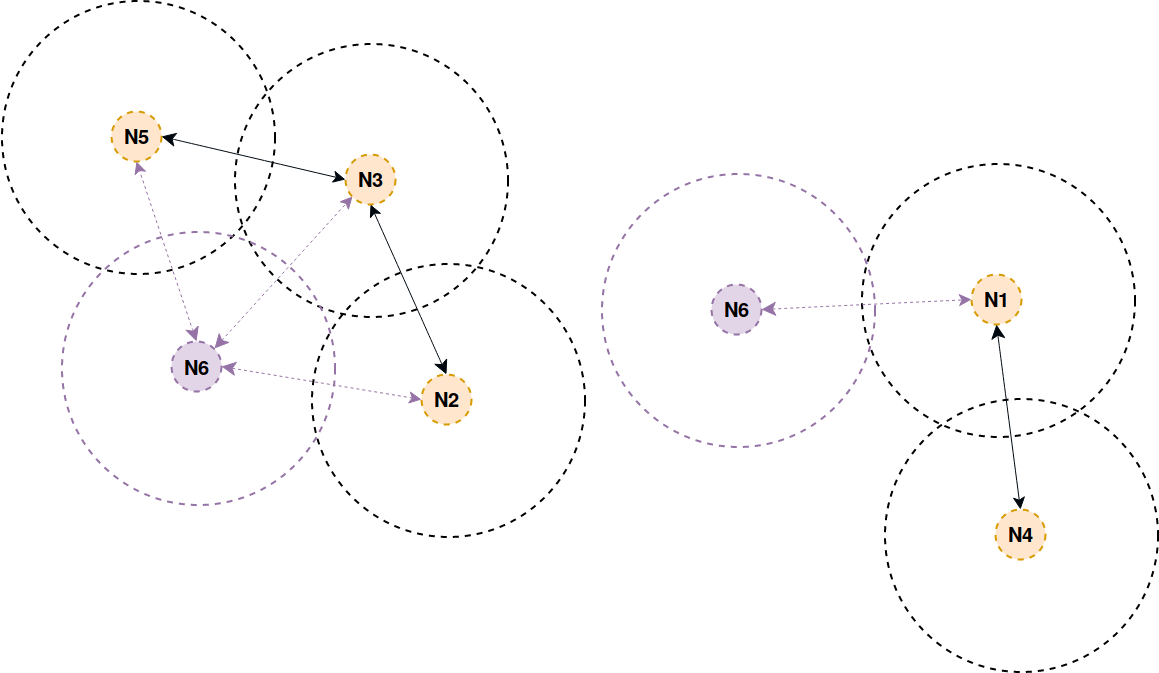
\includegraphics[width=\textwidth]{contactNewNeighbour.png}
%\caption{Figure show how new nodes (purple) contacts their neighbours.}
%\label{fig:contactNeighbour}
%\end{figure}


%\section{Maintenance Of Known Nodes}
\section{Cluster Head Election}
A \gls{ch} election may occur in two scenarios listed below.

%\begin{figure}
%\centering
%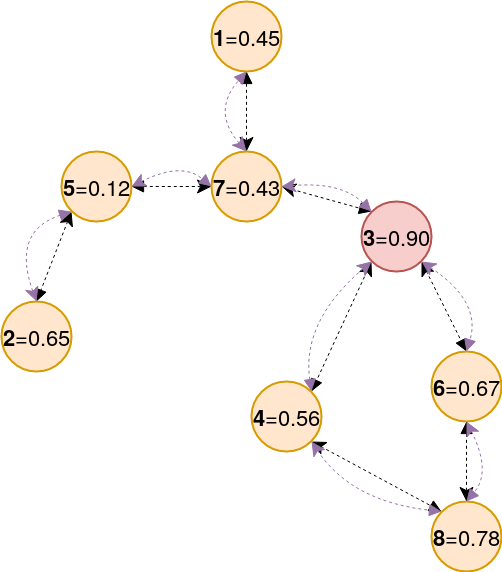
\includegraphics[width=\textwidth]{leaderElection.png}
%\caption{Figure show how a \gls{ch} election is gossiped in the cluster.}
%\label{fig:leaderElection}
%\end{figure}


\subsection{New Node In Cluster Starts Election}
When a new nodes has joined the cluster, it will start a new \gls{ch} election. It will calculate it's own \gls{ch}-score and gossip the score to its neighbours. The neighbours will then start a \gls{ch} election comparing the received \gls{ch}-score against it's own \gls{ch}-score. The result of the \gls{ch} election will then be gossiped to the nodes neighbours with either the received \gls{ch}-score or the nodes own \gls{ch}-score. The gossiped message also contains a path to the leader. The node append its own address to the path if the received \gls{ch}-score won the election, otherwise will the path to leader only contain the node itself. Eventually a new \gls{ch} is elected and consistent in the whole cluster. A \gls{ch} election is shown in Figure \ref{fig:newNodeLeaderElection}.

\begin{figure}
\centering
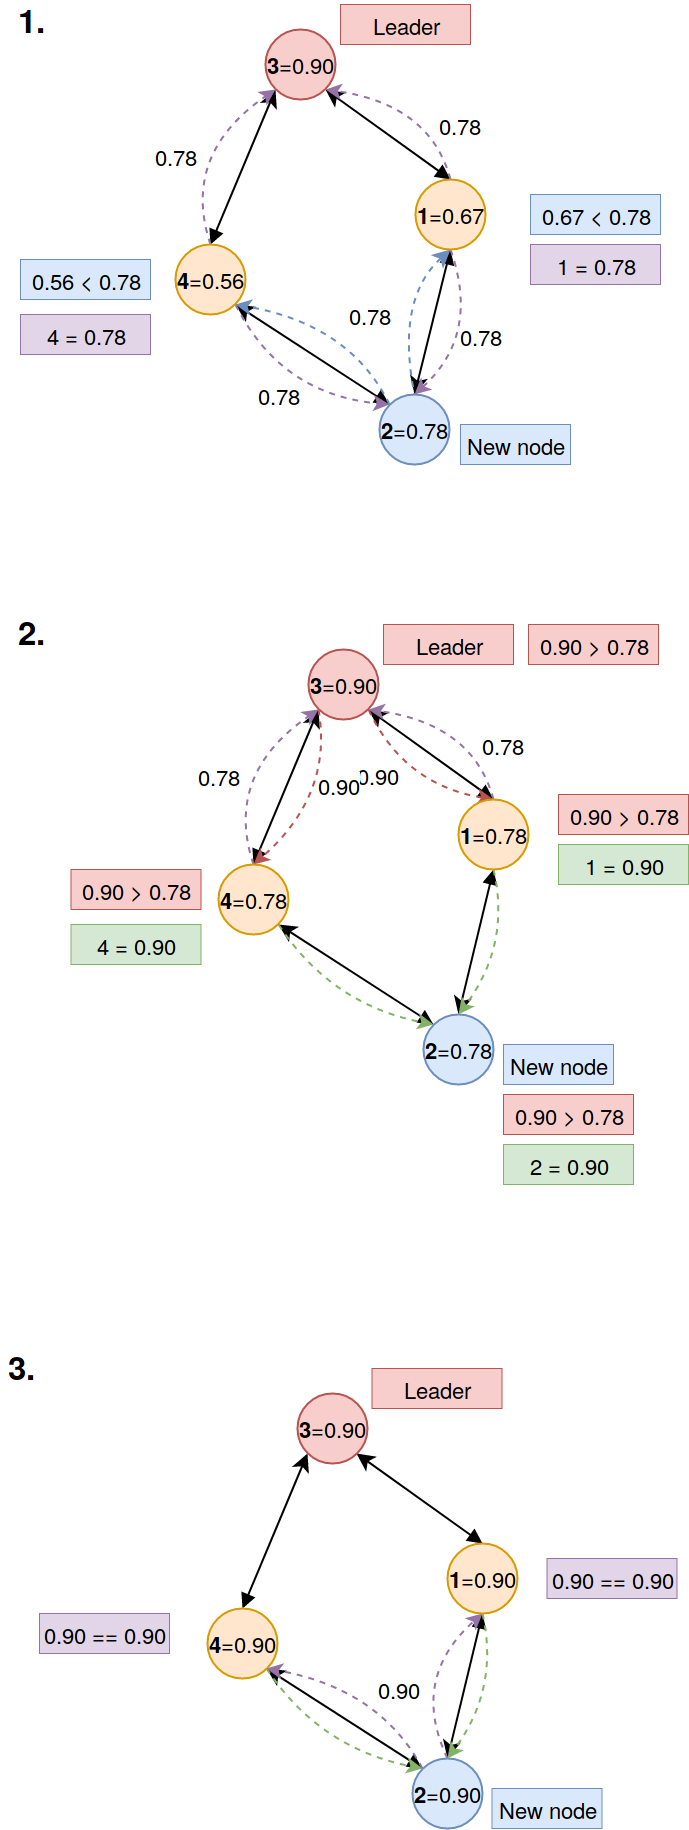
\includegraphics[scale=0.3]{newNodeLeaderElection.png}
\caption{Figure show how a new node starts a leader election.}
\label{fig:newNodeLeaderElection}
\end{figure}


\subsection{Cluster Head Starts Election}
When a \gls{ch} has accumulated data a certain times, it will start a new \gls{ch} election. Initially, the \gls{ch} will gossip a message to nodes the cluster to calculate a new \gls{ch}-score. Then it will the \gls{ch} start a new election and gossip this election to the other nodes. The nodes receiving this gossip message will start their leader-election as described in the section above. The election is illustrated in Figure \ref{fig:chWantsLeaderElection}.

\begin{figure}
\centering
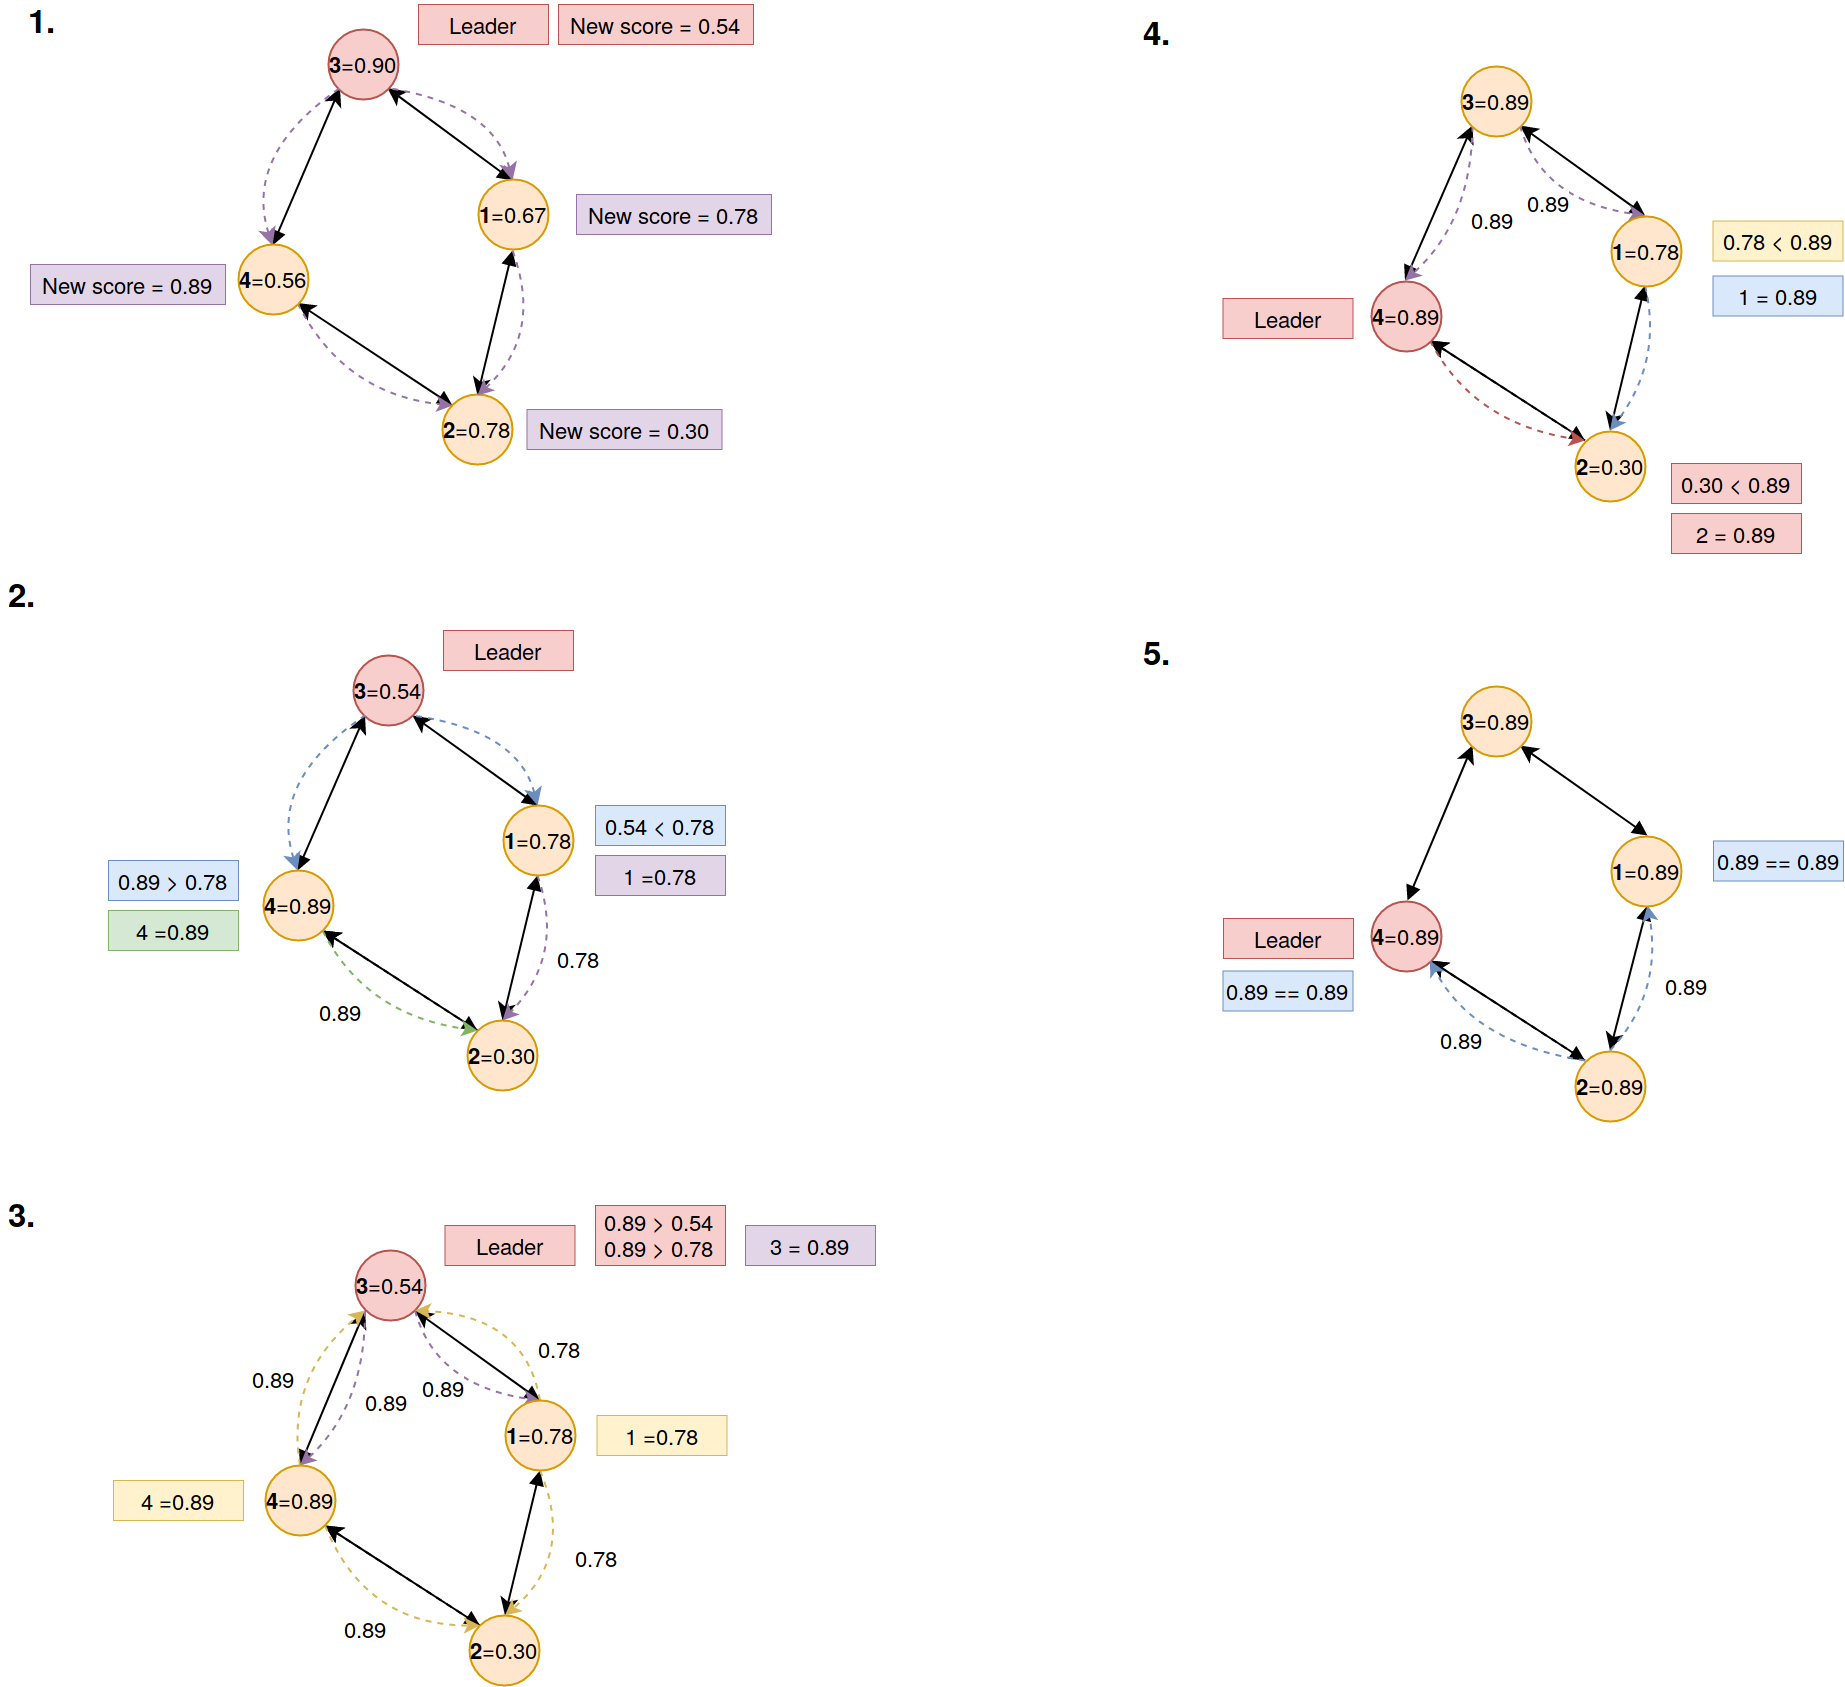
\includegraphics[width=\textwidth]{LeaderNewLeaderElection2.png}
\caption{Figure show how a new node starts a leader election.}
\label{fig:chWantsLeaderElection}
\end{figure}


\newpage

\section{Accumulate Data}
A node may at times forward data to another node in the cluster.

\begin{figure}
\centering
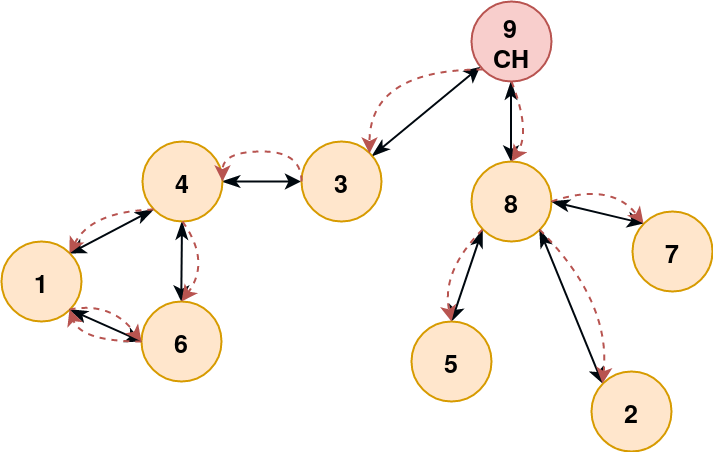
\includegraphics[width=\textwidth]{gatherData.png}
\caption{Figure show how nodes get an request for sending data to the leader.}
\label{fig:gatherData}
\end{figure}


%\section{Base Station Access?}
%CH will keep data and send it to BS when it has access??
%CH changes so not


%\newpage
%\begin{lstlisting}[frame=single,caption={Small C program},language=C]
%Code
%\end{lstlisting}



\chapter{Implementation}
%Threads, data structures, language

This chapter will elaborate on how we implemented the system, general implementation requirements, issues and choices. 
%We will first look at some libraries used in this implementation, then we will take a look at ... At last, we will describe the ...

The system is implemented in the open source programming language GO 1.9.3\footnote{\url{https://golang.org/}}.

%\section{Simulator}
%It is not feasible to have nodes out in the Arctic Tundra (like ZebraNet..) at such an early stage. This implementation simulates a real-life environment where nodes can 

\section{Distance To Other Nodes In The Network}

The formula \ref{eq:distance} is used to calculate the range between two points in a two-dimentional coordinate map and is used to see if a node is within a range or not, as seen in Figure \ref{fig:broadcast_range}.

\begin{equation} \label{eq:distance}
d = \sqrt{(X_{2} - X_{1})^{2}+(Y_{2} - Y_{1})^{2}}
\end{equation}

%node attempt to connect..

Figure \ref{fig:broadcast_simulation} shows how a node contact the lookup service where the nodes position is calculated and nodes in range is returned to the node. At last, the node will try to connect to the reachable nodes.

\begin{figure}
\centering
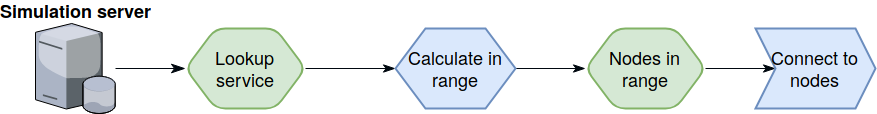
\includegraphics[width=\textwidth]{broadcast_simulation.png}
\caption{Broadcast simulation}
\label{fig:broadcast_simulation}
\end{figure}

\section{Data Transmission}
\subsection{Cluster Head Election}
%Leader election takes time to stabilize because of gossiping..
%Bully algorithm.. traditonially algorithm: nodes ON, we assume nodes OFF/our nodes ost likely OFF.. 
%Gossip-based peer sampling - acm - mark jelasity \cite{gbsampling}

\section{Minimize Path To Leader}
%Djikstra shortest path - Eclidean distance..

%\cite{multiradio}: The goal of the metric is to choose a high-throughput path between  a source  and  a  destination

\section{Data Accumulation}
%If leader election occurs at the same time that a leader is gathering data, get EOF when broadcasting.. But does not stop/exit program..

%Maps are not concurrent, need locks to prevent deadlock.. Or use a implementation of concurrent-map..

%mediated = try to bring to an agreement

The collected data is stored in a map and maps in Go are not safe for concurrent use. If a map is read from and wrote to from concurrent goroutines, the access must be compromised by a synchronization mechanism. One of the most common ways to protect maps is by using mutexes.
\begin{lstlisting}[frame=single,caption={Small Go program showing how mutexes are used when updating a map},language=C]
/*DBStation is a strucure that contains 
a map that store data at leader*/
var DBStation struct {
	sync.Mutex
	BSdatamap map[uint32][]byte
}

func sendDataToLeaderHandler() {
	DBStation.Lock()
	defer DataBaseStation.Unlock()
	
	...
	
	DBStation.BSdatamap[sData.FP] = receivedData
}
\end{lstlisting}



\chapter{Evaluation}
This chapter describes the experimental setup and metrics used to evaluate the implemented system.

\section{Experimental Setup}
All experiments were done on a Lenovo ThinkCenter with the following specifications:

\begin{itemize} 
\item Intel® CoreTM i5-6400T CPU @ 2.20GHz × 4
\item Intel® HD Graphics 530 (Skylake GT2)
\item 15,6 GiB memory and 503 GB disk
\item Ubuntu 17.04 64-bit with gcc V6.3.0 compiler and GO 1.9.3
\end{itemize}


\section{Experimental Design}
%\begin{table}[]
%\centering
%\label{my-label}
%\begin{tabular}{|l|l|}
%\hline
%\textbf{Parameter}       & \textbf{Value} \\ \hline
%No. of nodes             & 100            \\ \hline
%Network size             & 500 x 500      \\ \hline
%Node broadcast width     & 100            \\ \hline
%\end{tabular}
%\caption{Parameters of simulation}
%\end{table}

%How did we do the experiments?

%For hvert eksperiment bør du prøve å få fram: 
%- hva ønsker du å finne ut? 
%- hvordan måler du + hva måler du? 
%- hva gjør den delen av systemet som du måler? (leser fra disk, regner, sammenligner, koordinerer med andre osv)
%- Hva er metrikken (eks: operasjoner per sekund, minutter per oppgave osv)
%Det gjør det lettere for leseren å henge med. 

\subsection{CPU Measurements}
\subsection{Memory Measurements}
\subsection{Network (Socket) Usage}
\subsection{Network Lifetime?}


\section{Results}
%What does the results say?
\subsection{CPU Usage}
\subsection{Memory Usage}
\subsection{Network Usage}
\subsection{Network Lifetime?}


\chapter{Discussion}
%Idea, arch, design, results, other solutions, "arch has scale issue"..

This chapter discusses our approach, experience, how we solved the problem and why we chose the solution we ended up with..


\section{Availability of nodes in the system}
%When a node wants to join the cluster, should it ask the CH or should it join eitherway.. What if CH is sleeping (or busy) so that it's not reachable, or that nodes in the path to CH are sleeping (then how to contact CH?)..


\section{Cluster Head Election}
%Eventual/weak consistency with leader election.. Gossiping with an ID to check if node receive the msg before or not.. Updating leader..

%Gossiping is an excellent way to rapidly spread information among a large number of nodes using only local information. There is no central component where information is coordinated. However, it cannot guarantee that all nodes will receive the information \cite{demers}. One of the main advantages of a gossip based algorithm is its ability to scale.

%To avoid flooding the network (too much), each msg have an ID so that a node can check if it has received the same message before (+ if the leader number is similar). If it as been received earlier, the node doesn't need to forward the message because it has likely forwarded the message in an earlier gossip.

%"Being a clusster head is much more energy intensive than eing a non-cluster head node. if the clulster heads where chosen a priori adn fied through the system lifetime, these nodes would quickly use up their limited energy. Once the CH runs out of energy, it is no longer operational, and all the nodes that belong to the cluster lose communcation ability."

\subsection{Cluster Head Calculation/Rating}
%now random number, to approve and make it more realistic: number of nodes between CH and node, power left on device, bandwidth, prior history, traffic on node..

\section{Path To Leader}
%avoid flooding
\section{Data Transmission}
%What if multiple leaders gather data? Replication of data is good, but also aqcuire more memory.. Find a tradeoff.. Can use fingerprint to identify data..

%How to gather data? Receive a GET-post from BS or someone else telling the CH to accumulate/gather data or gather data periodically? How does a BS send a GET-request to CH?? The CH could not be in range of the BS, so maybe send to a node in range and forward msg all the way to CH.. But again, what if some nodes are sleeping to save battery? The CH will then not receive the msg..
\subsection{Data Accumulation}

\section{Base Station Access}

\chapter{Conclusion}
In this thesis, we have implemented a system/prototype...

Our experiments showed that the system ...
\chapter{Future Work}

\chapter{Appendix}


\backmatter

%%% BIBLOGRAPHY

\newpage{}

\begin{thebibliography}{9}
%1
\bibitem{leach}
W. R. Heinzelman and A. Chandrakasan and H. Balakrishnan,
\newblock {\em Energy-efficient communication protocol for wireless microsensor networks}, 2000,
\newblock in {\em Proceedings of the 33rd Annual Hawaii International Conference on System Sciences, 10 pp. vol.2-}.

%2 - ikke printet ut/ikke i bruk
%\bibitem{leach_perf}
%K. Latif and M. Jaffar and N. Javaid and M. N. Saqib and U. Qasim and Z. A. Khan,
%\newblock {\em Performance Analysis of Hierarchical Routing Protocols in Wireless Sensor Networks}, 2012,
%\newblock in {\em 2012 Seventh International Conference on Broadband, Wireless Computing, Communication and Applications, pp. 620-625}.

%3 ikke i bruk
%\bibitem{fuzzy_rule}
%K. Gotefode and K. Kolhe,
%\newblock {\em Energy efficiency in wireless sensor network using Fuzzy rule and tree based routing protocol}, 2015,
%\newblock in {\em 2015 International Conference on Energy Systems and Applications, pp. 712-717}.

%4
\bibitem{tree_based}
Z. Han and J. Wu and J. Zhang and L. Liu and K. Tian,
\newblock {\em A General Self-Organized Tree-Based Energy-Balance Routing Protocol for Wireless Sensor Network}, 2014,
\newblock in {\em IEEE Transactions on Nuclear Science Vol.61, Nr.2, pp. 732-740}.

%5 ikke i bruk
%\bibitem{routing_survey}
%J. N. Al-Karaki and A. E. Kamal,
%\newblock {\em Routing techniques in wireless sensor networks: a survey}, 2004,
%\newblock in {\em IEEE Wireless Communications Vol.11, Nr.6, pp. 6-28}.

%6
\bibitem{pegasis}
S. Lindsey and C. S. Raghavendra,
\newblock {\em PEGASIS: Power-efficient gathering in sensor information systems}, 2002,
\newblock in {\em Proceedings, IEEE Aerospace Conference Vol.3, pp. 3-1125-3-1130}.

%7 - ikke skrevet ut/ ikke i bruk
%\bibitem{atyp_routing}
%X. Liu,
%\newblock {\em Atypical Hierarchical Routing Protocols for Wireless Sensor Networks: A Review}, 2015,
%\newblock in {\em IEEE Sensors Journal Vol.15, Nr.10, pp. 5372-5383}.

%8
\bibitem{fuzzy_logic}
A. K. Mishra and R. Kumar and J. Singh,
\newblock {\em A review on fuzzy logic based clustering algorithms for wireless sensor networks}, 2015,
\newblock in {\em 2015 International Conference on Futuristic Trends on Computational Analysis and Knowledge Management (ABLAZE), pp. 489-494}.

%9
\bibitem{ch_fuzzy}
Indranil Gupta and D. Riordan and Srinivas Sampalli,
\newblock {\em Cluster-head election using fuzzy logic for wireless sensor networks}, 2005,
\newblock in {\em 3rd Annual Communication Networks and Services Research Conference (CNSR'05), pp. 255-260}.

%10
\bibitem{dec_cb_alg}
Maryam Sabet and Hamid Reza Naji,
\newblock {\em A decentralized energy efficient hierarchical cluster-based routing algorithm for wireless sensor networks}, 2015,
\newblock in {\em AEU - International Journal of Electronics and Communications Vol.69, Nr.5, pp. 790 - 799}.

%11 ikke i bruk
%\bibitem{rout_prot_survey}
%Shio Kumar Singh, M P Singh and D K Singh,
%\newblock {\em Routing Protocols in Wireless Sensor Networks – A Survey }, 2010,
%\newblock in {\em International Journal of Computer Science \& Engineering Survey (IJCSES) Vol.1, No.2, November 2010, pp. 63-83}.

%12
\bibitem{leach_c}
W. B. Heinzelman and A. P. Chandrakasan and H. Balakrishnan,
\newblock {\em An application-specific protocol architecture for wireless microsensor networks},
\newblock in {\em IEEE Transactions on Wireless Communications Vol.1, No.4, October 2002, pp. 660-670}.

%13 ikke i bruk
\bibitem{demers}
Demers, Alan and Greene, Dan and Hauser, Carl and Irish, Wes and Larson, John and Shenker, Scott and Sturgis, Howard and Swinehart, Dan and Terry, Doug,
\newblock {\em Epidemic algorithms for replicated database maintenance},
\newblock in {\em ACM: Proceedings of the Sixth Annual ACM Symposium on Principles of Distributed Computing, 1987, pp. 1--12}.

%14
\bibitem{leach_e}
Chen, Bai and Zhang, Yaxiao and Li, Yuxian and Hao, Xiao-Chen and Fang, Yan,
\newblock {\em A Clustering Algorithm of Cluster-head Optimization for Wireless Sensor Networks Based on Energy},
\newblock in {\em Journal of Information and Computational Science, Vol.8, 2011}.

%15
\bibitem{leach_b}
M. Tong and M. Tang,
\newblock {\em LEACH-B: An Improved LEACH Protocol for Wireless Sensor Network},
\newblock in {\em J2010 6th International Conference on Wireless Communications Networking and Mobile Computing (WiCOM), 2010, pp. 1-4}.

%16 ikke i bruk
\bibitem{zebranet}
Juang, Philo and Oki, Hidekazu and Wang, Yong and Martonosi, Margaret and Peh, Li Shiuan and Rubenstein, Daniel,
\newblock {\em Energy-efficient Computing for Wildlife Tracking: Design Tradeoffs and Early Experiences with ZebraNet},
\newblock in {\em ACM: SIGARCH Comput. Archit. News, Vol.30, No.5, December 2002, pp. 96--107}.

%17 ikke i bruk
%\bibitem{dataColl}
%Di Francesco, Mario and Das, Sajal K. and Anastasi, Giuseppe,
%\newblock {\em Data Collection in Wireless Sensor Networks with Mobile Elements: A Survey},
%\newblock in {\em ACM Trans. Sen. Netw., Vol.8, No.1, August 2011, pp. 7:1--7:31}.

%18 ikke i bruk
\bibitem{gbsampling}
Jelasity, M\'{a}rk and Voulgaris, Spyros and Guerraoui, Rachid and Kermarrec, Anne-Marie and van Steen, Maarten,
\newblock {\em Gossip-based Peer Sampling},
\newblock in {\em ACM Trans. Comput. Syst., Vol.25, No.3, August 2007}.

%19 ikke i bruk
\bibitem{multiradio}
Draves, Richard and Padhye, Jitendra and Zill, Brian,
\newblock {\em Routing in Multi-radio, Multi-hop Wireless Mesh Networks},
\newblock in {\em Proceedings of the 10th Annual International Conference on Mobile Computing and Networking, 2004, pp.114--128}.




\end{thebibliography}


\end{document}

